\section{Evaluation}

\subsection{User Feedback}
Once the prototype had been completed, we wanted to receive some user feedback on the general idea of Choona and the client side app. This feedback will help us determine whether or not the system so far satisfies its intended purpose. This testing has been carried out on a small group of participants that covered a broad customer base allowing us to gain useful feedback.  There were two feedback events; our demo presentation to our customer from Atos and one with potential Choona users.

\subsection{Demo}
We presented our prototype to Mike.  He was provided with a mobile device running the Choona app and asked to play around with the system.  We felt this would provide us with some useful feedback.  During the demo, the back end services crashed.  Although this was not what we expected to happen, the whole system relaunched itself without the need for interaction or manual input; showing the scalability and reliability of the micro-services infrastructure.  Apart from this small issue, the demonstration of the system was a success and we received good overall feedback.  Mike was impressed with the app design and felt the layout worked well with the concept of Choona.  On an overall level, he thought there was huge potential behind the idea and has recommended talking to other third party sources such as Sonos.

\subsubsection{Feedback conditions}
In our demo to potential users, we decided to make use of our Raspberry Pi adaptor to test its capabilities when there were multiple users interacting with the system at once. The app was then placed on everyone's mobile device. After the session was over, the participants were asked to complete a survey (created using survey monkey\footcite{survey}).

\subsubsection{Results}
There were a total of 17 participants; 10 male and 7 female. The age of these participants aired between 18 and 54. The highest number of participants were within the 18-24 category.
From the users feedback, we noticed a level split between the two major operating systems with Android being used by 35\% of the participants and iOS used by 40\% of participants.  This correlates with our findings during the literature review.  The participants spread for mobile device operating system.  \\
The participants generally seemed interested in music as shown in figure \ref{fig:interest_music}.  53\% were interested in music with 41\% very interested in music.  \\

    \begin{figure}[h!]
      \centering
      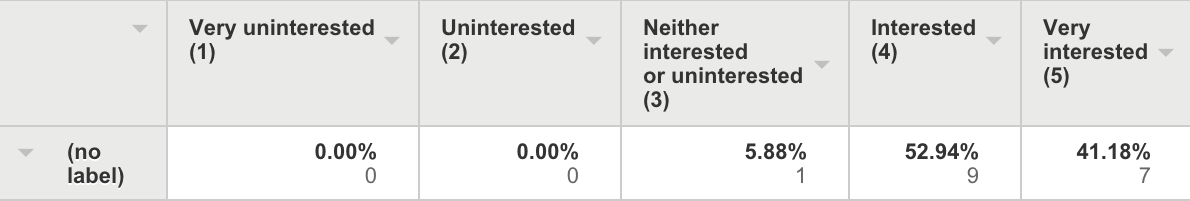
\includegraphics[width=0.8\textwidth]{./img/music_interest.png}
      \caption{Participants interest in music}
      \label{fig:interest_music}
    \end{figure}

The feedback we received for overall experience of Choona was very positive with 47\% very satisfied and 47\% satisfied with the majority of users happy with the look and feel of the app (59\%).  Navigation around the app was deemed easy (88\% of users).  \\
During our research, we discovered what makes a UI effective and we tried to incorporate this into the app.  This feedback has highlighted that we are along the right tracks and have a solid foundation.  However, with 2 individuals neither satisfied or unsatisfied with the look, feel and navigation, it shows we still have work to do.  One of the areas mentioned to us was the `up-vote/down-vote' buttons on the playlist - other ways to display this type of feature.  \\

We also asked for input on how often they would use Choona.  Just over 10\% came back and said they would use it extremely often (all the time).  Very often received 47\% of the vote and moderately often received 34\% of the vote.  These figures were slightly lower than we had hoped for. We were hoping for a slightly higher `extremely often' response.  This identifies to us that there will be different situations when a user feels they will be in a situation to use Choona but decide they won't want to.  Although this can be the case sometimes, we want users to be using Choona as much as possible.  We want the experience to be rewarding enough for them to constantly be using it.  Therefore, this has identified an area we can improve upon; to make Choona more applicable in any situation.  \\

    \begin{figure}[h!]
      \centering
      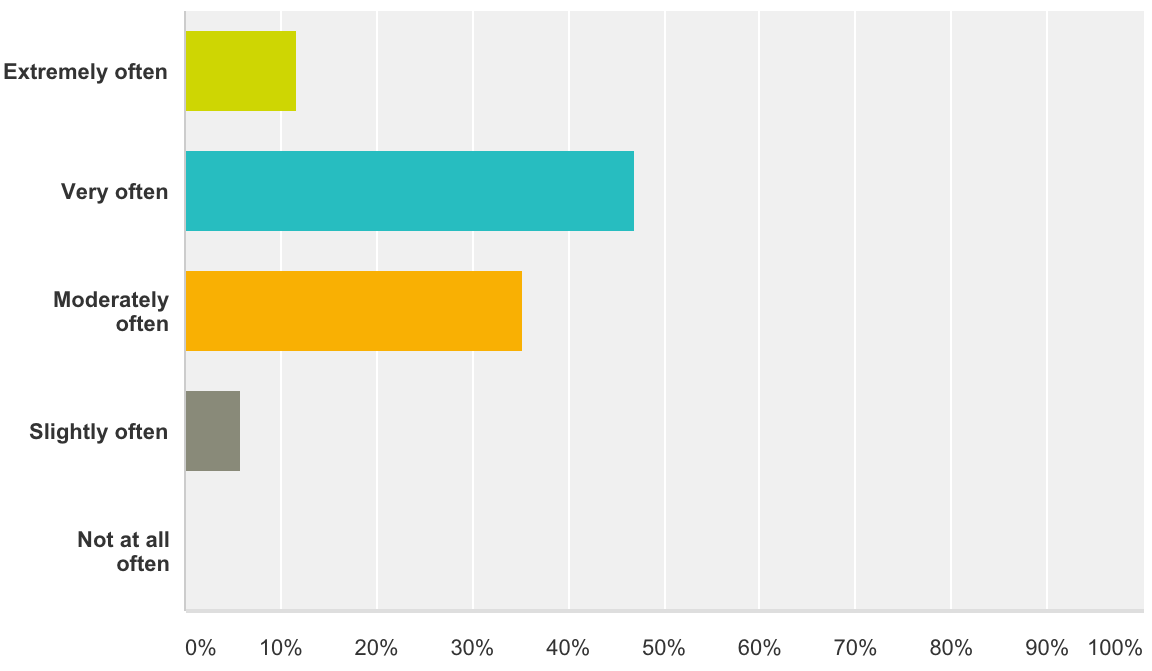
\includegraphics[width=0.8\textwidth]{./img/how_often.png}
      \caption{How often they would use Choona}
      \label{fig:how_often}
    \end{figure}

Linked to the previous question, participants were also asked when they would make use of Choona and the results are shown in figure \ref{fig:where}.  This highlights that the most popular options are coffee shops, bars/restaurants and nightclubs.  This is useful feedback as this will help us position our service in the right way to make sure we have a good initial user base. There wasn't an unanimous result for any one situation. This means the users are telling us that they all have different preferences for the use of Choona.  This is vital information and is something that we believe we need to work on.  We want to make sure that all scenarios fit with Choona.  \\

    \begin{figure}[h!]
      \centering
      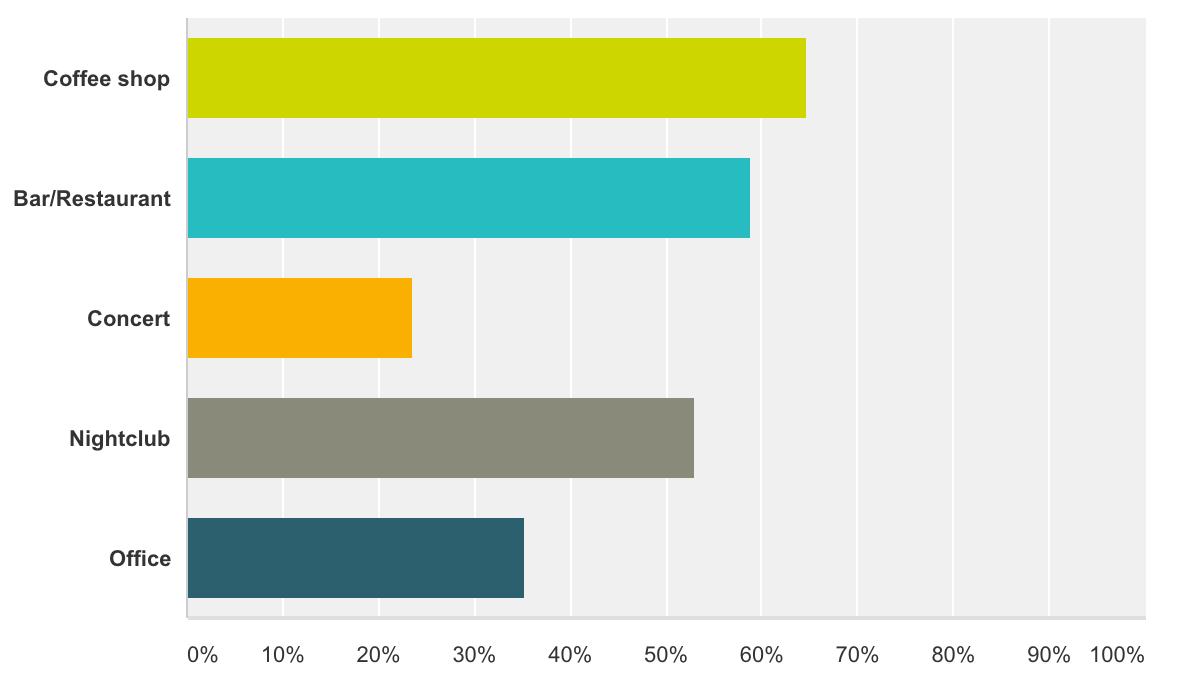
\includegraphics[width=0.8\textwidth]{./img/use_situation.png}
      \caption{Where they would use Choona}
      \label{fig:where}
    \end{figure}

The final question was whether or not the participant would recommend Choona to friends or family.  All seventeen participants said `yes'.  This feedback signifies that we have come up with a service that actually provides value to a customer and something that is significant enough to recommend to other people.

\subsubsection{Conclusion}
There are several different pieces of information that we can take from this feedback session.  Firstly, the overall feedback about Choona is positive; a unique idea filling a gap in the market and confirmation that the app itself is a good basis to work from.  We need to go away and make some fundamental changes; design including buttons and layout but all features within the app received positive feedback with no one indicating that a feature was redundant.  We did receive some comments that reflected additional features we could add to the app such as a `current charts' page.  This would show the most played songs over a week long period and could include a `Choona chart' where this shows the most popular songs across the entire choose network or a top chart for a particular franchise e.g. a Starbucks chart list.  The results of the recommendation of Choona question is something that will provide motivation to move further ahead with this project.

\subsection{Market Readiness}

The Choona prototype has proved that the idea itself works as a technical system and is well received by users, however there are still several important milestones to complete before Choona is be ready to release to the general public.

\begin{itemize}
  \item \textbf{Audio Licensing and Partnerships}\\
    We've previously discussed the issues surrounding music licensing for public locations and how they can be resolved, however another hurdle that will have to be tackled is the restrictions that many audio sources have in their terms of service. Spotify, for example, has a blanket ban on using their service in any commercial or non-personal environment\footcite{spotifypublic} with the exception of official partnership agreements\footcite{spotifypartners}. This is most likely going to be the case for most, if not all, online music services, meaning we will have to approach each company on a case-by-case basis with a partnership proposal. On the surface this may just seem like a business development issue, however it could also have an impact on Choona's software as well. For example, Spotify might require their own logo and advertising to be embedded in the app which will require additional development work and integration with third party systems.

    There is also a possibility that rival music services would not be happy with Choona supporting them both; it is highly unlikely that Spotify will endorse and enter a partnership agreement with a product that is also in a partnership with Google Music, especially if the product is still in the prototype stages. Therefore in order to get to get to market in a reasonable time frame it may be necessary to focus on partnering with one or two main services initially.

  \item \textbf{Client Management Interface}\\
    Choona currently has no management systems or interfaces for clients to manage their accounts. We plan to implement a separate mobile application and access API called Fishtank, designed purely for use by clients and not the general public. It is becoming increasingly common for large multi-context applications to break their apps down into multiple single-context apps; Facebook's release of their separate Pages Manager\footcite{facebookpages} is an excellent example. Having separate applications helps to keep code bases leaner and allows you to update more frequently with less chance of breaking other functionality.

    Fishtank will offer a wide range of management options to clients:
    \begin{itemize}
      \item \textit{Geofence manipulation}: designation of geofences at verified Choona locations.
      \item \textit{User management}: ability to ban users, give them rewards etc.
      \item \textit{Playlist settings}: configure default playlists to load when the user-managed queue is empty, restrict searching to only pull from a subset of available tracks, define content restrictions on available songs (such as explicit content exclusion), select different upvote/downvote algorithms to use.
      \item \textit{Playlist override}: ability to skip songs on the fly, pause the entire stream, bump a song to the top of the queue.
      \item \textit{Ad/offer management}: insertion of visual adverts into various placeholders of the Choona application (e.g. playlist banner), creating and integrating audio adverts into the Choona stream, target offers and adverts to specific subsets of users (e.g. give frequent users a discount).
      \item \textit{Speaker adapter settings}: control the output volume, select different geolocations.
    \end{itemize}

    Without Fishtank it will be hard to appeal to enterprise clients that will be looking for a polished, well-rounded system that is easy to set up and control.

  \item \textbf{User accounts}\\
    We currently do not maintain any server-side data about users. This means it is impossible to store long-term data such as listening history or user access levels. In order to make this happen a database service needs to be created that will be responsible for storing account data. This will be accessible via a dedicated user service that is responsible for combining profile data from Auth0 with context-specific data from the Choona user database, as shown in figure \ref{fig:user-service}.

    \begin{figure}[h!]
      \centering
      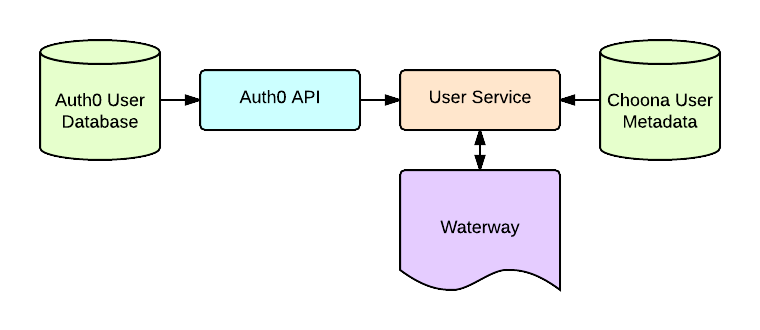
\includegraphics[width=0.8\textwidth]{./img/userservice.png}
      \caption{Future user service}
      \label{fig:user-service}
    \end{figure}

  \item \textbf{Infrastructure improvements and testing}\\
    The majority of the code used in the prototype is not currently covered by unit tests, making it unsafe for proper production use. Every service in the Choona infrastructure needs to have 100\% code coverage before being officially released. Furthermore every aspect of the system needs to be stress tested to ensure it is capable of supporting a high number of users. This will most likely require load balancing of certain resource-intensive services such as the Socket.IO API and the Spotify source that directly interface and manipulate audio data.
\end{itemize}
